% =====================================================================
\chapter{Matemática de bolso}\label{cap:03}
\naaula{09 a 16}

Este capítulo reúne toda a matemática de que você vai precisar, explicada do zero. Não pule
nenhuma seção, mesmo que o assunto pareça conhecido: cada uma termina ligando a ideia a algo que
você já programou.

% ---------------------------------------------------------------------
\section{Funções: uma máquina de entrada e saída}

Uma \textbf{função} é uma regra que recebe um valor de entrada e devolve um valor de saída. Pense
numa máquina: você coloca um número de um lado e sai um número do outro.

\begin{figure}[!htb]
\centering
\begin{tikzpicture}[font=\large]
  \node[draw=edteal, fill=edtealclaro, line width=1.2pt, rounded corners=3pt,
        minimum width=3.2cm, minimum height=1.4cm] (m) at (0,0) {$T(n) = 3n + 4$};
  \node[anchor=east] (e) at (-3.4,0) {$n = 5$};
  \node[anchor=west] (s) at (3.4,0) {$T(5) = 19$};
  \draw[-{Latex[length=3mm]}, line width=1.2pt, edverde] (e) -- (m);
  \draw[-{Latex[length=3mm]}, line width=1.2pt, edlaranja] (m) -- (s);
  \node[font=\small, color=edcinza] at (-2.6,-1.0) {entrada: o tamanho};
  \node[font=\small, color=edcinza] at (2.8,-1.0) {saída: os passos};
\end{tikzpicture}
\caption{A função $T(n) = 3n + 4$, que conta os passos da soma de um vetor (capítulo 2).}
\end{figure}

Escrevemos $T(n)$ para dizer \enquote{o valor de $T$ quando a entrada é $n$}. Para calcular, basta
trocar $n$ pelo número: $T(5) = 3 \cdot 5 + 4 = 19$. Em análise de algoritmos, a entrada $n$ é
quase sempre o \textbf{tamanho} dos dados — o mesmo número que o \codigo{tamanho()} da nossa Lista
devolve — e a saída é o \textbf{custo}: passos, comparações, deslocamentos.

\subsection{Tabela e gráfico}

Uma função pode ser mostrada como tabela ou como gráfico. No gráfico, cada ponto tem duas
coordenadas: a posição na horizontal é a entrada $n$; a altura é a saída $T(n)$.

\begin{center}
\begin{tabularx}{0.85\textwidth}{P{3.2cm} C C C C C C}
\cab \tcx{$n$} & \tc{0} & \tc{1} & \tc{2} & \tc{5} & \tc{8} & \tc{10} \\
$T(n) = 3n + 4$ & 4 & 7 & 10 & 19 & 28 & 34 \\
\end{tabularx}
\end{center}

\begin{figure}[!htb]
  \centering
  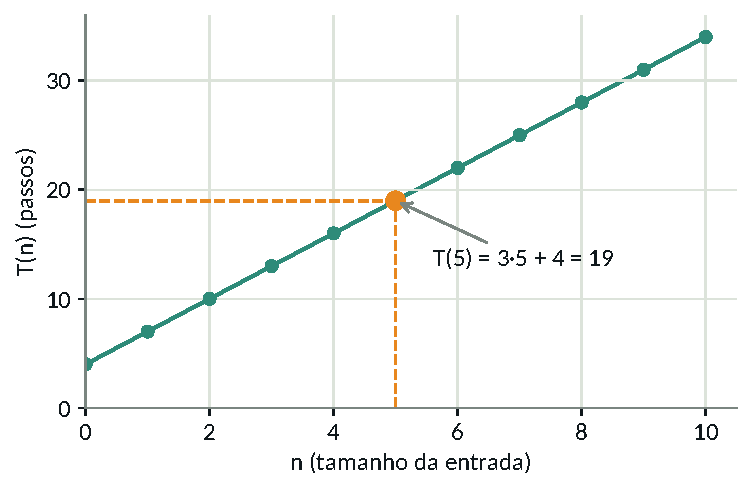
\includegraphics[width=0.66\textwidth]{figuras/f03_grafico_3n4.pdf}
  \caption{Como ler um gráfico: ande na horizontal até $n = 5$, suba até a linha e olhe a altura
  à esquerda: 19.}
\end{figure}

% ---------------------------------------------------------------------
\section{Funções crescentes}

Uma função é \textbf{crescente} quando, ao aumentar a entrada, a saída nunca diminui. Em
símbolos: se $a < b$, então $f(a) \le f(b)$. O custo de um algoritmo é (quase sempre) uma função
crescente: mais dados, mais trabalho. O que muda de um algoritmo para outro é \textbf{a
velocidade} com que o custo cresce.

\begin{figure}[!htb]
  \centering
  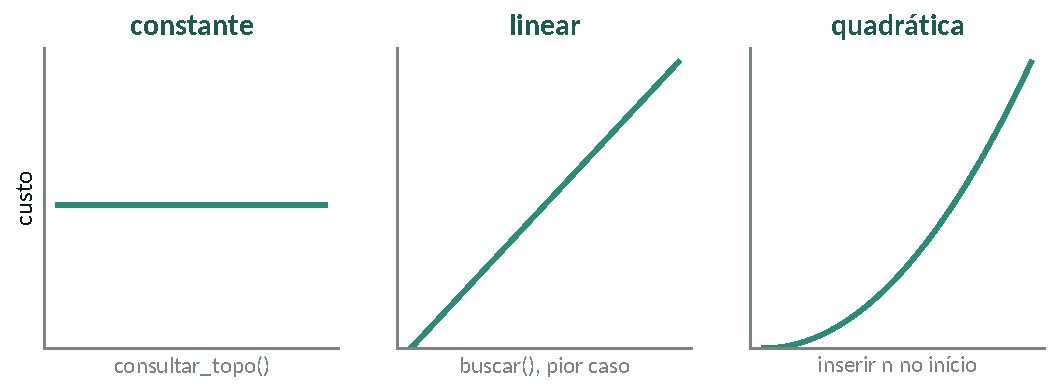
\includegraphics[width=0.95\textwidth]{figuras/f03_tipos_crescimento.pdf}
  \caption{Três formas de crescer, com exemplos das Aulas 1 e 2.}
\end{figure}

\begin{itemize}
  \item \textbf{Constante:} o custo não depende de $n$. O \codigo{consultar_topo()} da Pilha
        custa o mesmo com 3 ou com 3 milhões de elementos. (Uma função constante conta como
        crescente no sentido de que \enquote{nunca diminui}.)
  \item \textbf{Linear:} o custo cresce na mesma proporção de $n$. Dobrou $n$, dobrou o custo.
        É o caso da busca linear quando o valor não está na lista.
  \item \textbf{Quadrática:} o custo cresce muito mais rápido. Dobrou $n$, o custo
        quadruplica. É o caso de inserir $n$ elementos, um a um, no início de uma lista contígua.
\end{itemize}

\begin{exrapido}
Considere $f(n) = 7$, $g(n) = 2n + 1$ e $h(n) = n^2$. (a) Calcule as três para $n = 1$, $5$ e
$10$. (b) Em cada caso, qual é a maior? (c) O que isso sugere sobre comparar funções olhando só
valores pequenos de $n$?
\end{exrapido}

% ---------------------------------------------------------------------
\section{Potências e raízes}

A \textbf{potência} $n^k$ é $n$ multiplicado por ele mesmo $k$ vezes: $n^2 = n \cdot n$ (lê-se
\enquote{ene ao quadrado}) e $n^3 = n \cdot n \cdot n$ (\enquote{ene ao cubo}). Os nomes vêm da
geometria: $n^2$ é a área de um quadrado de lado $n$; $n^3$, o volume de um cubo.

\begin{figure}[!htb]
\centering
\begin{tikzpicture}[scale=0.55]
  \foreach \x in {0,...,3} \foreach \y in {0,...,3}
    \draw[fill=edtealclaro, draw=edteal, line width=0.8pt] (\x,\y) rectangle ++(1,1);
  \node[font=\small] at (2,-0.6) {lado $n = 4$};
  \node[font=\small, rotate=90] at (-0.6,2) {lado $n = 4$};
  \node[font=\large, anchor=west] at (4.8,2.6) {$n^2 = 4 \times 4 = 16$ casas};
  \node[font=\small, anchor=west, color=edcinza, align=left] at (4.8,1.2)
    {como um tabuleiro de Campo Minado $4 \times 4$,\\ou uma matriz guardada numa lista contígua};
\end{tikzpicture}
\caption{$n^2$ conta as casas de um quadrado de lado $n$.}
\end{figure}

A \textbf{raiz quadrada} faz o caminho inverso: $\sqrt{n}$ é o lado de um quadrado com $n$ casas.
$\sqrt{16} = 4$, $\sqrt{100} = 10$, $\sqrt{10.000} = 100$. Também se escreve $\sqrt{n} = n^{1/2}$.

\subsection{Regras que vamos usar}

\begin{center}
\begin{tabularx}{\textwidth}{P{3.6cm} P{3.8cm} L}
\cab \tc{Regra} & \tc{Exemplo} & \tc{Em palavras} \\
$n^a \cdot n^b = n^{a+b}$ & $2^3 \cdot 2^4 = 2^7 = 128$ & multiplicar: soma os expoentes \\
\rowcolor{edfundo} $(n^a)^b = n^{a \cdot b}$ & $(n^2)^3 = n^6$ & potência de potência: multiplica \\
$n^1 = n$ \quad e \quad $n^0 = 1$ & $7^0 = 1$ & qualquer número (não nulo) elevado a 0 dá 1 \\
\rowcolor{edfundo} $n^{-1} = \dfrac{1}{n}$ & $10^{-2} = \dfrac{1}{100}$ & expoente negativo: inverte \\
$n^{1/2} = \sqrt{n}$ & $64^{1/2} = 8$ & expoente ½ é a raiz quadrada \\
\end{tabularx}
\end{center}

\begin{conexao}
Na Aula 3, a interseção \enquote{ingênua} de dois Conjuntos com $n$ e $m$ elementos perguntava,
para cada elemento do primeiro, se ele pertencia ao segundo: $n$ consultas de custo $m$, ou
seja, $n \cdot m$ comparações. Se os dois têm o mesmo tamanho, isso dá $n^2$.
\end{conexao}

\begin{exrapido}
Calcule: (a) $2^3 \cdot 2^4$; (b) $\sqrt{64}$; (c) $(n^2)^3$; (d) $10^{-2}$; (e) $1.000^{1/3}$
(dica: que número multiplicado por ele mesmo 3 vezes dá 1.000?).
\end{exrapido}

% ---------------------------------------------------------------------
\section{Logaritmos: quantas vezes dá para dividir ao meio?}

Pegue 16 caixas e vá dividindo ao meio até sobrar uma. Quantas divisões são necessárias?

\begin{figure}[!htb]
\centering
\begin{tikzpicture}[scale=0.42]
  \foreach \linha/\qtd in {0/16, 1/8, 2/4, 3/2, 4/1} {
    \foreach \i in {1,...,\qtd}
      \draw[fill=edtealclaro, draw=edteal, line width=0.7pt] (\i-1, -\linha*1.5) rectangle ++(0.85,0.85);
    \node[anchor=west, font=\small] at (16.4, -\linha*1.5+0.42) {\textbf{\qtd}};
  }
  \foreach \linha/\num in {0/1, 1/2, 2/3, 3/4}
    \node[font=\small, color=edlaranja, anchor=west] at (18.4, -\linha*1.5-0.33) {$\div 2$ \ (divisão \num)};
\end{tikzpicture}
\caption{$16 \to 8 \to 4 \to 2 \to 1$: são 4 divisões. Por isso, $\log_2 16 = 4$.}
\end{figure}

O número de divisões ao meio até chegar a 1 é o \textbf{logaritmo na base 2}. Escrevemos
$\log_2 16 = 4$ (lê-se \enquote{logaritmo de 16 na base 2 é 4}). Olhando ao contrário: dobrando
4 vezes a partir de 1, chegamos a 16, ou seja, $2^4 = 16$. Esta é a definição:

\begin{center}
\colorbox{edtealclaro}{\large\quad $\log_2 n = x \quad\Longleftrightarrow\quad 2^x = n$\quad}
\end{center}

\begin{center}
\begin{tabularx}{\textwidth}{L C C C C C C C}
\cab \tcx{$n$} & \tc{1} & \tc{2} & \tc{8} & \tc{16} & \tc{1.024} & \tc{1.048.576} & \tc{≈ 1 bilhão} \\
$\log_2 n$ & 0 & 1 & 3 & 4 & 10 & 20 & $\approx 30$ \\
\end{tabularx}
\end{center}

Repare no mais importante: quando $n$ vai de mil para um milhão (mil vezes mais), o logaritmo só
vai de 10 para 20. \textbf{O logaritmo cresce muito devagar.} Um algoritmo que faz $\log_2 n$
passos é excelente.

\begin{intuicao}
O jogo \enquote{adivinhe o número de 1 a 100}: a cada palpite, você ouve \enquote{maior} ou
\enquote{menor}. Chutando sempre o meio, cada resposta elimina metade dos números que sobram. Em
no máximo 7 palpites você acerta, porque $2^7 = 128 \ge 100$. Esse é o princípio da
\emph{busca binária} em um vetor ordenado: cerca de $\log_2 n$ comparações.
\end{intuicao}

\subsection{E quando \texorpdfstring{$n$}{n} não é uma potência de 2?}

O logaritmo continua existindo, só que não é inteiro: $\log_2 1.000 \approx 9{,}97$, porque
$2^{9{,}97} \approx 1.000$. Para calcular numa calculadora (ou no Python), use:

\[
\log_2 n = \frac{\ln n}{\ln 2} \approx 3{,}32 \cdot \log_{10} n
\qquad\text{no Python: } \texttt{math.log2(n)}
\]

\subsection{Propriedades úteis}

\begin{center}
\begin{tabularx}{\textwidth}{P{4.2cm} P{4.4cm} L}
\cab \tc{Propriedade} & \tc{Exemplo} & \tc{Em palavras} \\
$\log(a \cdot b) = \log a + \log b$ & $\log_2 (8 \cdot 4) = 3 + 2 = 5$ & produto vira soma \\
\rowcolor{edfundo} $\log(n^k) = k \cdot \log n$ & $\log_2 (2^{10}) = 10$ & o expoente \enquote{desce} \\
$\log 1 = 0$ & $\log_2 1 = 0$ & porque $2^0 = 1$ \\
\rowcolor{edfundo} $\log_2 n = 3{,}32 \cdot \log_{10} n$ & $\log_2 1.000 \approx 3{,}32 \cdot 3$ & bases diferentes só diferem por uma constante \\
\end{tabularx}
\end{center}

\begin{atencao}
A última propriedade tem uma consequência importante: em análise de algoritmos, a base do
logaritmo \textbf{não importa}. Trocar de base só multiplica o resultado por uma constante — e
constantes são desprezadas (capítulo 4). Por isso escrevemos simplesmente $O(\log n)$.
\end{atencao}

\begin{figure}[!htb]
  \centering
  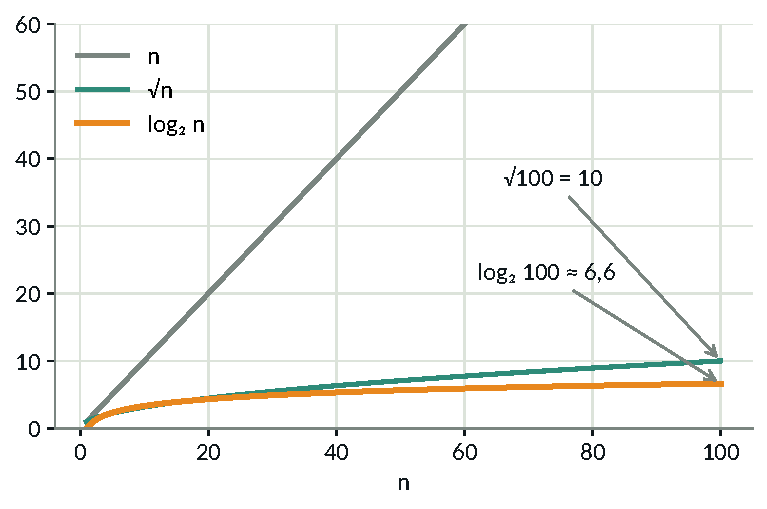
\includegraphics[width=0.7\textwidth]{figuras/f03_log_raiz.pdf}
  \caption{Para $n = 100$: $n$ vale 100, $\sqrt{n}$ vale 10 e $\log_2 n$ vale só 6,6.}
\end{figure}

\begin{exrapido}
(a) $\log_2 64$; (b) $\log_2 1.024$; (c) entre quais inteiros está $\log_2 100$?
(d) Quantas vezes é preciso dividir 1.000.000 ao meio para chegar a 1 (aproximadamente)?
\end{exrapido}

% ---------------------------------------------------------------------
\section{Exponenciais: dobrar a cada passo}

Na \textbf{exponencial} $2^n$, a variável está no expoente: cada vez que $n$ aumenta 1, o valor
\textbf{dobra}. $2^{10} = 1.024$, $2^{20} \approx$ um milhão, $2^{30} \approx$ um bilhão.

\begin{intuicao}
Diz a lenda que o inventor do xadrez pediu como prêmio 1 grão de trigo na primeira casa do
tabuleiro, 2 na segunda, 4 na terceira, dobrando até a casa 64. Parece pouco, mas a última casa
sozinha teria $2^{63}$ grãos, e o total, $2^{64} - 1 \approx 1{,}8 \times 10^{19}$ grãos —
muito mais trigo do que o mundo inteiro já produziu.
\end{intuicao}

Onde a exponencial aparece em computação? Sempre que um algoritmo testa \textbf{todas as
combinações} de escolhas do tipo sim/não.

\begin{conexao}
Um Conjunto (Aula 3) com $n$ elementos tem $2^n$ subconjuntos. Para cada elemento, há duas
escolhas: ele está no subconjunto ou não. São $2 \times 2 \times \dots \times 2 = 2^n$ combinações.
Para $\{A, B, C\}$:

\begin{center}
\begin{tabularx}{0.9\linewidth}{C C C L}
\cab \tc{A está?} & \tc{B está?} & \tc{C está?} & \tc{Subconjunto} \\
não & não & não & $\varnothing$ (vazio) \\
\rowcolor{white} não & não & sim & $\{C\}$ \\
não & sim & não & $\{B\}$ \\
\rowcolor{white} não & sim & sim & $\{B, C\}$ \\
sim & não & não & $\{A\}$ \\
\rowcolor{white} sim & não & sim & $\{A, C\}$ \\
sim & sim & não & $\{A, B\}$ \\
\rowcolor{white} sim & sim & sim & $\{A, B, C\}$ \\
\end{tabularx}
\end{center}

São $2^3 = 8$ subconjuntos. Com 30 elementos, seriam mais de um bilhão.
\end{conexao}

\begin{figure}[!htb]
  \centering
  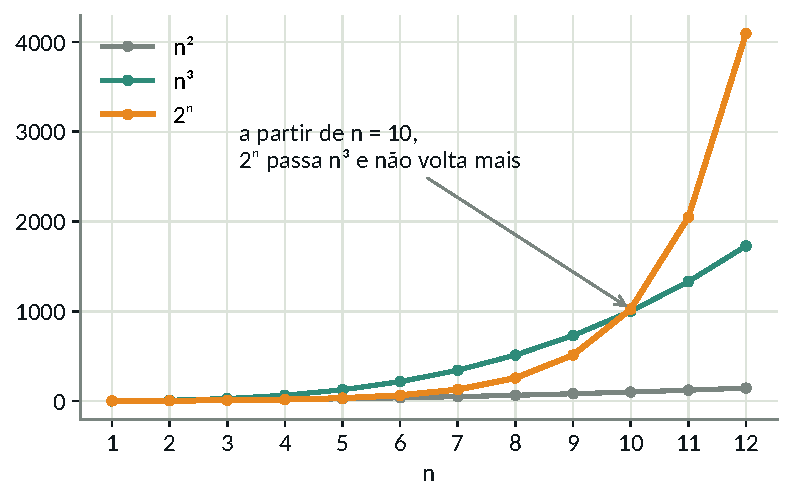
\includegraphics[width=0.7\textwidth]{figuras/f03_exponencial.pdf}
  \caption{No começo, $2^n$ parece inofensiva: fica abaixo de $n^3$ até $n = 9$. A partir de
  $n = 10$, passa à frente e dispara.}
\end{figure}

% ---------------------------------------------------------------------
\section{Fatorial: todas as ordens possíveis}

O \textbf{fatorial} de $n$, escrito $n!$ (lê-se \enquote{ene fatorial}), é o produto de todos os
inteiros de 1 até $n$:
\[
n! = n \times (n-1) \times \dots \times 2 \times 1,
\qquad 3! = 3 \cdot 2 \cdot 1 = 6, \qquad 5! = 120, \qquad 0! = 1 \text{ (por convenção)}.
\]

O fatorial conta de quantas \textbf{ordens} diferentes podemos arrumar $n$ objetos.

\begin{conexao}
Na central de impressão da Aula 2, três trabalhos — 101, 102 e 103 — podem chegar à fila em
qualquer ordem. Para o primeiro lugar, há 3 opções; escolhido o primeiro, sobram 2 para o
segundo; e o último fica com a única que resta: $3 \times 2 \times 1 = 6$ ordens.
\end{conexao}

\begin{figure}[!htb]
\centering
\begin{tikzpicture}[
  level 1/.style={sibling distance=4.4cm, level distance=1.25cm},
  level 2/.style={sibling distance=2.1cm, level distance=1.25cm},
  level 3/.style={level distance=1.1cm},
  every node/.style={font=\small, draw=edteal, fill=edtealclaro, rounded corners=2pt, inner sep=3pt},
  edge from parent/.style={draw=edteal, line width=0.8pt}]
  \node[fill=edteal, text=white] {início}
    child {node {101}
      child {node {102} child {node[fill=white] {103}}}
      child {node {103} child {node[fill=white] {102}}}}
    child {node {102}
      child {node {101} child {node[fill=white] {103}}}
      child {node {103} child {node[fill=white] {101}}}}
    child {node {103}
      child {node {101} child {node[fill=white] {102}}}
      child {node {102} child {node[fill=white] {101}}}};
\end{tikzpicture}
\caption{As $3! = 6$ ordens de chegada de três trabalhos à fila de impressão. Cada caminho do
início até uma folha é uma ordem.}
\end{figure}

\begin{center}
\begin{tabularx}{\textwidth}{L C C C C C}
\cab \tcx{$n$} & \tc{3} & \tc{5} & \tc{10} & \tc{15} & \tc{20} \\
$2^n$ & 8 & 32 & 1.024 & 32.768 & $\approx 1$ milhão \\
\rowcolor{edfundo} $n!$ & 6 & 120 & 3.628.800 & $\approx 1{,}3 \times 10^{12}$ & $\approx 2{,}4 \times 10^{18}$ \\
\end{tabularx}
\end{center}

O fatorial cresce ainda mais rápido que a exponencial: a partir de $n = 4$ ($4! = 24 > 2^4 = 16$),
passa à frente e nunca mais é alcançado. Um algoritmo que testa todas as ordens possíveis de $n$
itens é inviável já para $n$ em torno de 20.

\begin{exrapido}
(a) Liste os subconjuntos de $\{A, B, C\}$ sem olhar a tabela. (b) Calcule $4!$. (c) De quantas
formas 4 trabalhos podem chegar à fila? (d) Calcule $\dfrac{5!}{3!}$ sem calcular os fatoriais
inteiros.
\end{exrapido}

% ---------------------------------------------------------------------
\section{Somatórios e a soma de Gauss}

Muitos algoritmos fazem um trabalho que cresce a cada volta de um laço: 1 passo na primeira volta,
2 na segunda, 3 na terceira\dots\ Para somar isso tudo, usamos o \textbf{somatório}, escrito com a
letra grega $\Sigma$ (sigma maiúsculo):

\[
\sum_{i=1}^{n} i \;=\; 1 + 2 + 3 + \dots + n
\]

Leia assim: \enquote{a soma de $i$, para $i$ indo de 1 até $n$}. O número embaixo diz onde o
contador começa; o de cima, onde termina; e a expressão ao lado diz o que somar em cada volta —
exatamente como um laço \codigo{for}:

\begin{lstlisting}
total = 0
for i in range(1, n + 1):   # i vai de 1 até n
    total = total + i       # soma a expressão "i"
\end{lstlisting}

Mais exemplos: $\sum_{i=1}^{4} i = 1 + 2 + 3 + 4 = 10$ \quad e \quad
$\sum_{i=1}^{3} 2i = 2 + 4 + 6 = 12$.

\subsection{O truque de Gauss}

Conta-se que, criança, Carl Friedrich Gauss recebeu a tarefa de somar os números de 1 a 100 e
respondeu em segundos: 5.050. Ele percebeu que, escrevendo a soma de trás para a frente embaixo
dela mesma, cada coluna soma sempre 101:

\[
\begin{array}{r@{\;}c@{\;}c@{\;}c@{\;}c@{\;}c@{\;}c@{\;}c@{\;}c}
      & 1   & + & 2   & + & \cdots & + & 100 & \\
  +   & 100 & + & 99  & + & \cdots & + & 1   & \\ \hline
      & 101 & + & 101 & + & \cdots & + & 101 & = 100 \times 101
\end{array}
\]

Isso é o dobro da soma pedida; então a soma é $\dfrac{100 \times 101}{2} = 5.050$. Em geral:

\begin{center}
\colorbox{edtealclaro}{\large\quad $\displaystyle \sum_{i=1}^{n} i \;=\; 1 + 2 + \dots + n \;=\; \frac{n(n+1)}{2}$\quad}
\end{center}

\begin{figure}[!htb]
\centering
\begin{tikzpicture}[scale=0.62]
  \foreach \c in {1,...,5} \foreach \r in {1,...,\c}
    \draw[fill=edtealclaro, draw=edteal, line width=0.8pt] (\c-1, \r-1) rectangle ++(1,1);
  \foreach \c in {1,...,5} \foreach \r in {\c,...,5}
    \draw[fill=edlaranjaclaro, draw=edlaranja, line width=0.8pt] (\c-1, \r) rectangle ++(1,1);
  \node[font=\small] at (2.5,-0.6) {$n = 5$ colunas};
  \node[font=\small, rotate=90] at (-0.7,3) {$n + 1 = 6$ linhas};
  \node[font=\small, anchor=west] at (6.0,4.2) {\textcolor{edteal}{\textbf{escada verde:}} $1 + 2 + 3 + 4 + 5$};
  \node[font=\small, anchor=west] at (6.0,3.2) {\textcolor{edlaranja}{\textbf{escada laranja:}} a mesma, virada};
  \node[font=\small, anchor=west, align=left] at (6.0,1.8) {juntas: retângulo $5 \times 6 = 30$\\uma só: $30 \div 2 = 15$};
\end{tikzpicture}
\caption{A prova visual de Gauss: duas escadas iguais formam um retângulo $n \times (n+1)$.}
\end{figure}

Duas variações que aparecem muito:
\[
\sum_{i=0}^{n-1} i \;=\; 0 + 1 + \dots + (n-1) \;=\; \frac{(n-1)\,n}{2}
\qquad\text{e}\qquad
\sum_{i=1}^{n} c \;=\; c \cdot n \quad \text{(somar a constante } c\text{, } n \text{ vezes).}
\]

\begin{conexao}
Lembra do exercício 3 da Aula 1 (\enquote{contando deslocamentos})? Inserir $n$ elementos, um a
um, sempre no início de uma lista contígua: o primeiro não desloca ninguém; o segundo desloca 1;
o terceiro, 2; \dots; o último, $n - 1$. Total: $0 + 1 + \dots + (n - 1) = \dfrac{n(n-1)}{2}$
deslocamentos. Para $n = 100$, são 4.950.
\end{conexao}

\begin{exrapido}
(a) $1 + 2 + \dots + 100$. (b) Inserindo 10, 20, 30, 40 e 50, sempre no início de uma lista
contígua vazia, quantos deslocamentos ocorrem ao todo? (c) E para $n = 100$ inserções?
(d) Quanto vale $2 + 4 + 6 + \dots + 2n$? (Dica: coloque o 2 em evidência.)
\end{exrapido}

% ---------------------------------------------------------------------
\section{Para \texorpdfstring{$n$}{n} muito grande}

A análise de algoritmos se interessa pelo que acontece quando $n$ fica \textbf{muito grande} —
milhões, bilhões. Escrevemos $n \to \infty$ (lê-se \enquote{ene tende ao infinito}) para dizer
\enquote{$n$ crescendo sem parar}. Veja o que acontece com duas divisões:

\begin{center}
\begin{tabularx}{\textwidth}{P{2.8cm} C C C C}
\cab \tcx{$n$} & \tc{10} & \tc{100} & \tc{1.000} & \tc{1.000.000} \\
$\dfrac{3n + 4}{n}$ & 3,4 & 3,04 & 3,004 & 3,000004 \\
\rowcolor{edfundo} $\dfrac{n^2}{2^n}$ & 0,098 & $\approx 7{,}9 \times 10^{-27}$ & praticamente 0 & praticamente 0 \\
\end{tabularx}
\end{center}

A primeira divisão se aproxima de 3: para $n$ grande, $3n + 4$ se comporta como \enquote{3 vezes
$n$}, e o $+4$ deixa de importar. A segunda se aproxima de 0: $2^n$ cresce tão mais rápido que
$n^2$ fica insignificante perto dela. Dizemos que a primeira \enquote{tende a 3} e a segunda
\enquote{tende a 0}. Essa é a ideia intuitiva de \textbf{limite}, que volta no capítulo 11 — e é
exatamente o que o próximo capítulo explora.

\begin{respostas}
  \resp{3.1} (a) $n = 1$: $f = 7$, $g = 3$, $h = 1$. $n = 5$: $f = 7$, $g = 11$, $h = 25$.
  $n = 10$: $f = 7$, $g = 21$, $h = 100$. (b) Para $n = 1$, a maior é $f$; para $n = 5$ e
  $n = 10$, é $h$. (c) Quem começa na frente pode terminar atrás: comparar algoritmos com $n$
  pequeno engana. O que importa é o comportamento para $n$ grande.

  \begin{center}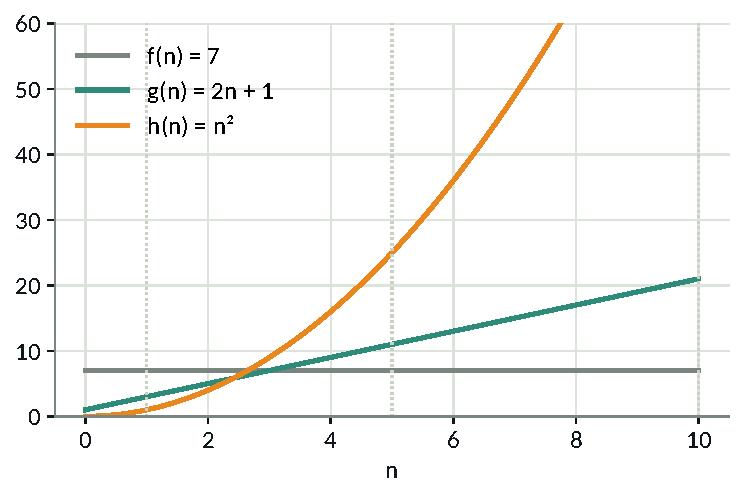
\includegraphics[width=0.6\textwidth]{figuras/f03_fgh.pdf}\end{center}

  \resp{3.2} (a) $2^7 = 128$. (b) 8. (c) $n^6$. (d) $\dfrac{1}{100} = 0{,}01$. (e) 10, porque
  $10 \times 10 \times 10 = 1.000$.
  \resp{3.3} (a) 6, pois $2^6 = 64$. (b) 10. (c) Entre 6 e 7, pois $2^6 = 64 < 100 < 128 = 2^7$
  (o valor exato é $\approx 6{,}64$). (d) Cerca de 20 vezes, pois $2^{20} \approx 1.000.000$.
  \resp{3.4} (a) $\varnothing$, $\{A\}$, $\{B\}$, $\{C\}$, $\{A,B\}$, $\{A,C\}$, $\{B,C\}$ e
  $\{A,B,C\}$: são 8. (b) $4! = 24$. (c) 24 formas. (d) $\dfrac{5 \cdot 4 \cdot 3!}{3!} = 5 \cdot 4 = 20$.
  \resp{3.5} (a) $\dfrac{100 \cdot 101}{2} = 5.050$. (b) $0 + 1 + 2 + 3 + 4 = 10$, que é
  $\dfrac{5 \cdot 4}{2}$. (c) $\dfrac{100 \cdot 99}{2} = 4.950$.
  (d) $2 + 4 + \dots + 2n = 2(1 + 2 + \dots + n) = 2 \cdot \dfrac{n(n+1)}{2} = n(n+1)$.
\end{respostas}
